\documentclass{article}
\usepackage{amssymb,graphicx,cancel}
\usepackage[margin=2cm]{geometry}
\usepackage{graphicx,epsfig,psfrag,bm,amssymb}
\usepackage{dcolumn}
\usepackage{bm}
\usepackage{color}
\usepackage{mathrsfs,amsfonts,hepunits,color}
\usepackage[utf8]{inputenc}
\usepackage{epsfig,latexsym,cancel,amssymb,amsmath,mathrsfs}
\usepackage{graphicx}
\usepackage{epstopdf}
\usepackage{mciteplus}
\usepackage{latexsym}
\usepackage{amsthm}
\usepackage{amsmath}
\usepackage{amssymb}
\usepackage{hepunits}
\usepackage{hyperref}
\usepackage{bbm}
\usepackage{bm}
\usepackage{xfrac}
\usepackage{color}
\usepackage{colordvi}
\usepackage{comment}
\usepackage{dcolumn}
\usepackage{times,latexsym,graphicx,wrapfig}
\usepackage{epsfig,lineno,bm}
\usepackage{subfigure}
\usepackage{slashed}

\begin{document}
\newcommand{\be}{\begin{eqnarray}}
\newcommand{\ee}{\end{eqnarray}}
\newcommand{\Gev}{\,\,\mathrm{GeV}}
\newcommand{\SUWeak}{\mathrm{SU}(2)_{\rm W}}
\newcommand{\Lag}{\mathcal{L}}
\newcommand{\Lagtree}{\mathcal{L}_{\rm tree}}
\newcommand{\benum}{\begin{enumerate}}
\newcommand{\eenum}{\end{enumerate}}
\newcommand{\bi}{\begin{itemize}}
\newcommand{\ei}{\end{itemize}}
\newcommand{\met}{\slashed{E_T}}
\newcommand{\ap}{{A^\prime}}


\title{LDMX Physics Motivation}
\maketitle
\section{Dark Matter Overview}
The overwhelming evidence for the existence of dark matter (DM) arises from multiple independent sources. 
 Observations of galactic rotation curves, the power spectrum of the Cosmic Microwave Background (CMB), 
the cosmological matter power spectrum, light element yields from Big Bang Nucleosynthesis (BBN), gravitational
lensing, and galaxy cluster collisions all require roughly 85\% of the matter in our universe to be cold and non-baryonic. 
Together, these data constitute smoking gun evidence  of physics beyond the Standard Model (SM), which contains
no viable DM candidate -- for a review see \cite{Bertone:2004pz}.

However, despite this impressive body of evidence, the particle nature of DM remains completely unknown; all indications of 
its existence derive ultimately from its gravitational influence on visible matter in different contexts. 
Without making any further assumptions about these hypothetical interactions or DM's cosmological history,
 its viable mass range is wildly unconstrained: $10^{-22} $ eV -- $10 M_{\odot}$.  If DM is lighter than $\sim 10^{-22}$ eV, 
 its Compton wavelength does not fit inside the smallest known DM dominated objects \cite{Navarro:1995iw} and if it's heavier than $\sim 10 M_{\odot}$ 
 it would have distorted the CMB power spectrum at early times \cite{Bird:2016dcv}. Given such an enormous range of viable masses, a realistic DM discovery effort requires a well motivated organizing principle to manageably and systematically test this vast space of possibilities without being narrowly tailored
 to specific models.

\subsection{Thermal Origin}
A compelling, well motivated organizing principle for the DM search effort is the hypothesis that DM
is produced through its interactions with the SM in thermal equilibrium during the early universe. This criterion
selects a broad class of popular DM models (including Supersymmetry) and is defined by the requirement that the DM-SM 
interaction rate exceed the Hubble expansion rate at early times.  
Once achieved, thermal equilibrium offers some generically attractive features that do not depend sensitively
on particular model details:
\begin{itemize}
\item {\bf Generically Realized:} Equilibrium is hard to avoid even with tiny coupling constants  between 
dark and visible matter; thus, most {\it discoverable} models of DM with non-gravitational interactions fall into this category. 
Alternative mechanisms (e.g. axions produced via misalignment \cite{Visinelli:2009zm} or feebly coupled DM produced via freeze in \cite{Hall:2009bx}) require such small couplings
that comprehensive experimental probes are prohibitively difficult in most regions of their parameter space -- see \cite{Essig:2013lka}.
\item {\bf Minimum Annihilation Rate:}  Equilibrium at temperature $T$ populates the DM with a  thermal number density $n_{\rm DM} \propto T^3$, which is many orders of magnitude larger than the observed abundance. Thus, viable thermal DM must be depleted with an annihilation cross section $\sigma v \ge 3\times10^{-26}$ cm$^3$/s via
the process of thermal ``freeze out." This inequality must be saturated (=) if DM is particle/antiparticle symmetric and exceeded ($>$)  if there is an additional primordial DM asymmetry which contributes to the total abundance in addition to the freeze-out component.

\item {\bf Narrower Mass Window: }The viable DM mass range becomes much narrower -- see Fig. \ref{fig:schematic}.
Thermal DM below $\lesssim$ 10 keV erases small scale structure in conflict with observation; 
thermal DM above $\gtrsim$ 10 TeV requires nonperturbative and/or non-unitary couplings to realize
a sufficiently large annihilation rate. 
\end{itemize}

\subsection{``WIMP" Dark Matter}
If thermal DM is realized in the upper half of the thermal mass window $\sim$ GeV - 10 TeV, it can be a Weakly Interacting Massive Particle (WIMP) charged under the 
familiar electroweak force and achieve the observed
relic abundance by annihilating through via SM gauge interactions.  This class of models exploits the numerical
 coincidence between electroweak-sized cross sections and the requisite annihilation cross section for thermal freeze out $\sigma \sim \alpha^2 /m_Z^2  \to \sigma v \sim 3 \times 10^{-26}$ cm$^3$/s (see \cite{Kolb:1990vq} for a pedagogical treatment). This so-called ``WIMP miracle" also naturally arises in popular extensions of the SM that address the electroweak hierarchy problem 
(e.g. Supersymmetry and extra dimensions) and may even be realized with fifth forces beyond the SM so long as the appropriate coupling-to-mass
ratio is of electroweak size, but the latter possibility is not obligatory for masses in the WIMP range.  




\begin{figure}[t!]
\center
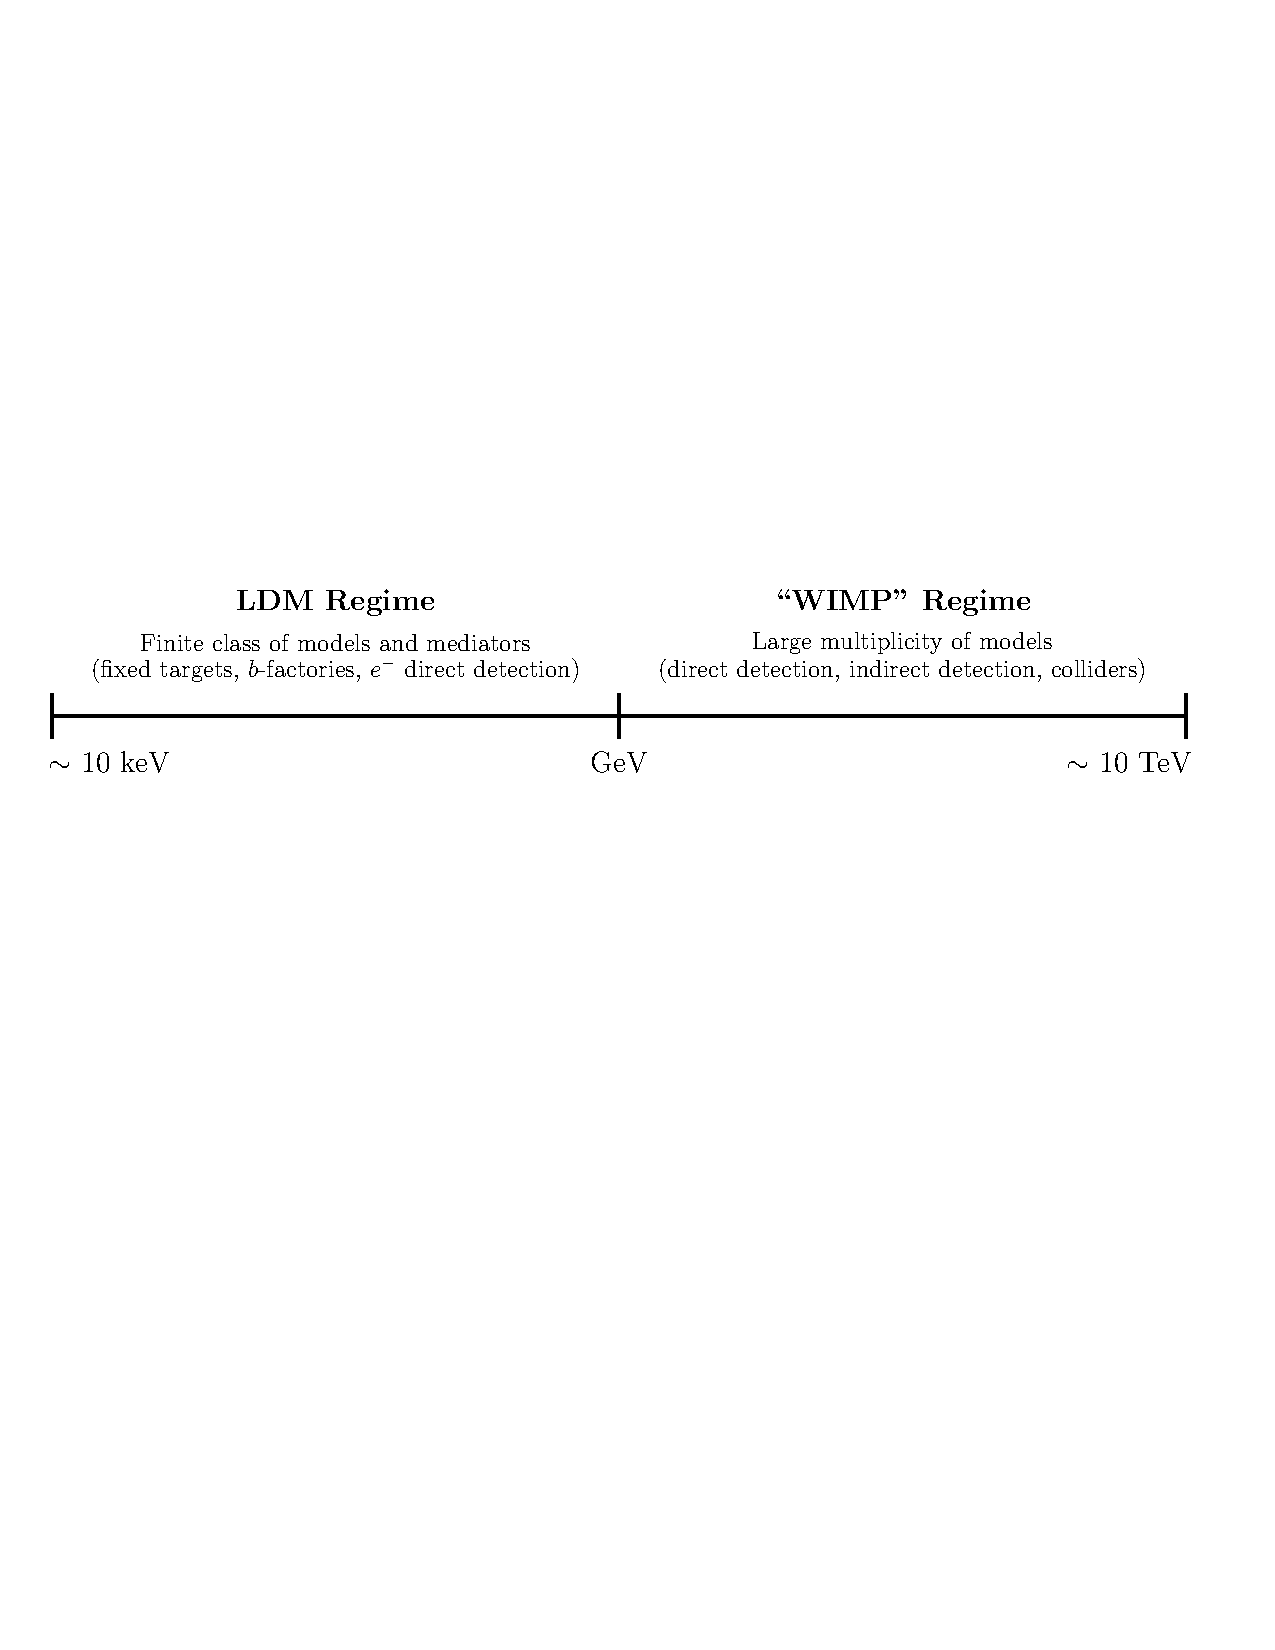
\includegraphics[width=15cm]{schematic.pdf}
\caption{The allowed mass range over which DM can thermalize with the SM in the early universe and yield the observed relic abundance via 
annihilation. For masses below $\lesssim 10$ keV, DM is too hot to form the observed structure of the universe on large scales  \cite{Viel:2013apy} and for masses above $\gtrsim 10$ TeV, a perturbative annihilation rate cannot achieve the correct relic abundance in simple models \cite{Griest:1989wds}. }
\label{fig:schematic}
\end{figure}

The discovery techniques available for WIMP and WIMP-like DM are well known and firmly established the experimental community:
\begin{itemize}
\item {\bf Direct Detection:} Terrestrial searches for non relativistic WIMP-nucleon scattering in a shielded underground detector \cite{Undagoitia:2015gya}. This technique 
is powerful for DM masses near $\sim$ 10 GeV - 10 TeV, but loses sensitivity near the GeV where typical nuclear recoils are $\lesssim$ keV,
below detection sensitivity thresholds. The sensitivity of this approach depends critically on the presently unknown DM velocity distribution in the 
terrestrial neighborhood and is therefore subject to potentially large systematic uncertainties. 

\item {\bf Indirect Detection:} Typically space based searches of DM annihilation in regions of high DM density (galactic center, dwarf galaxies etc.) \cite{Conrad:2014tla}.
This technique is approaching sensitivity to thermal DM annihilation rates for a variety of scenarios, but poorly constrains DM below the 
few-GeV scale. As with direct detection, the signal strength for indirect detection depends on an unknown DM phase space profile in regions of high density, 
so the systematic uncertainties of this approach may also be very large. 

\item {\bf Collider Production} Laboratory based searches for DM produced in association with visible final states in SM particle collisions \cite{Askew:2014kqa}. This technique
is powerful and not limited by halo uncertainties or the limitations of non-relativistic scattering off DM particles in the Earth's neighborhood. However, 
for DM below the GeV scale, the transverse missing energy in a typical production evennt is too low to impart sufficient recoil $P_T$ to the other
visible object(s) in the final state, so sensitivities remain weak for the lower half of the thermal mass window \cite{Izaguirre:2015yja}. 

\end{itemize}

\subsection{Light Dark Matter (LDM)}

Although the thermal freeze-out production mechanism can apply equally well to light DM (LDM) in the keV-GeV range, 
achieving the observed annihilation rate is no longer possible with SM forces. Annihilation to SM particles via virtual electroweak gauge boson exchange
scales as $\sigma v \sim \alpha^2 m_{\rm DM}^2/m_Z^4 \ll 3\times 10^{-26} $ cm$^3$/s, which is insufficient for freeze out if $m_{\rm DM} \ll m_{Z}$. Thus,
for light thermal DM to be viable:
\begin{itemize}
\item {\bf Light New Forces:} There have to be comparably light force carriers with to mediate an efficient  annihilation rate 
for thermal freeze out. 
\item {\bf Portals: } Both the DM and the mediator must be singlets under the full SM gauge group; otherwise 
 would have been produced in Z-pole measurements at LEP. Thus, in order for the DM to annihilate away its abundance, the mediator particle 
 must have a {\it renormalizable}\footnote{If the operator were not renormalizable, 
 there would have to be additional, sub-electroweak states integrated out to generate 
 such an interaction since electroweak sized suppression scales in higher dimension operators would reintroduce 
 the overproduction problem. However, the states that UV complete such an interaction would be 
 electroweak charged and ruled out by LEP searches for light, electroweak charged matter. } coupling to SM particles through a mass-dimension $< 4$ singlet ``portal" operator built out of SM fields.
\end{itemize}
The second bullet point sharply constrains the options for LDM mediator particles since the only renormalizable SM operators that
satisfy this requirement are 
\be
\hat {\cal O}_{\rm portal}   =  H^\dagger H  ~~,~~   H L ~~~, ~~~ B_{\mu\nu} ~~,~~
\ee
and are known respectively as the Higgs, lepton, and vector portals (for a discussion, see \cite{Pospelov:2008zw}). Here $H$ is the SM Higgs doublet, $L$ is the SM lepton doublet, and 
$B_{\mu \nu } = \partial_\mu B_\nu - \partial_\nu B_\mu$ is the $U(1)_Y$ hypercharge field strength tensor, which is independently gauge invariant. 
Each portal corresponds to a different choice of mediator spin -- only a scalar mediator can couple to the $H^\dagger H$ bilinear, only a fermionic mediator can couple to 
the lepton portal operator $LH$, and only a spin-1 mediator can couple to the $B_{\mu \nu}$ vector portal.
However, for the most predictive model variations, the scalar mediator is strongly disfavored by a variety of experimental constraints \cite{Krnjaic:2015mbs} 
and the lepton portal interaction is generically proportional to factors of neutrino masses $m_\nu \lesssim 0.1$ eV, so it is difficult to sustain 
thermal contact between DM and SM sectors. Thus, for the rest of this discussion, we will emphasize the vector portal as the representative mediator1
of LDM interactions. 

\begin{figure}[t!]
\center
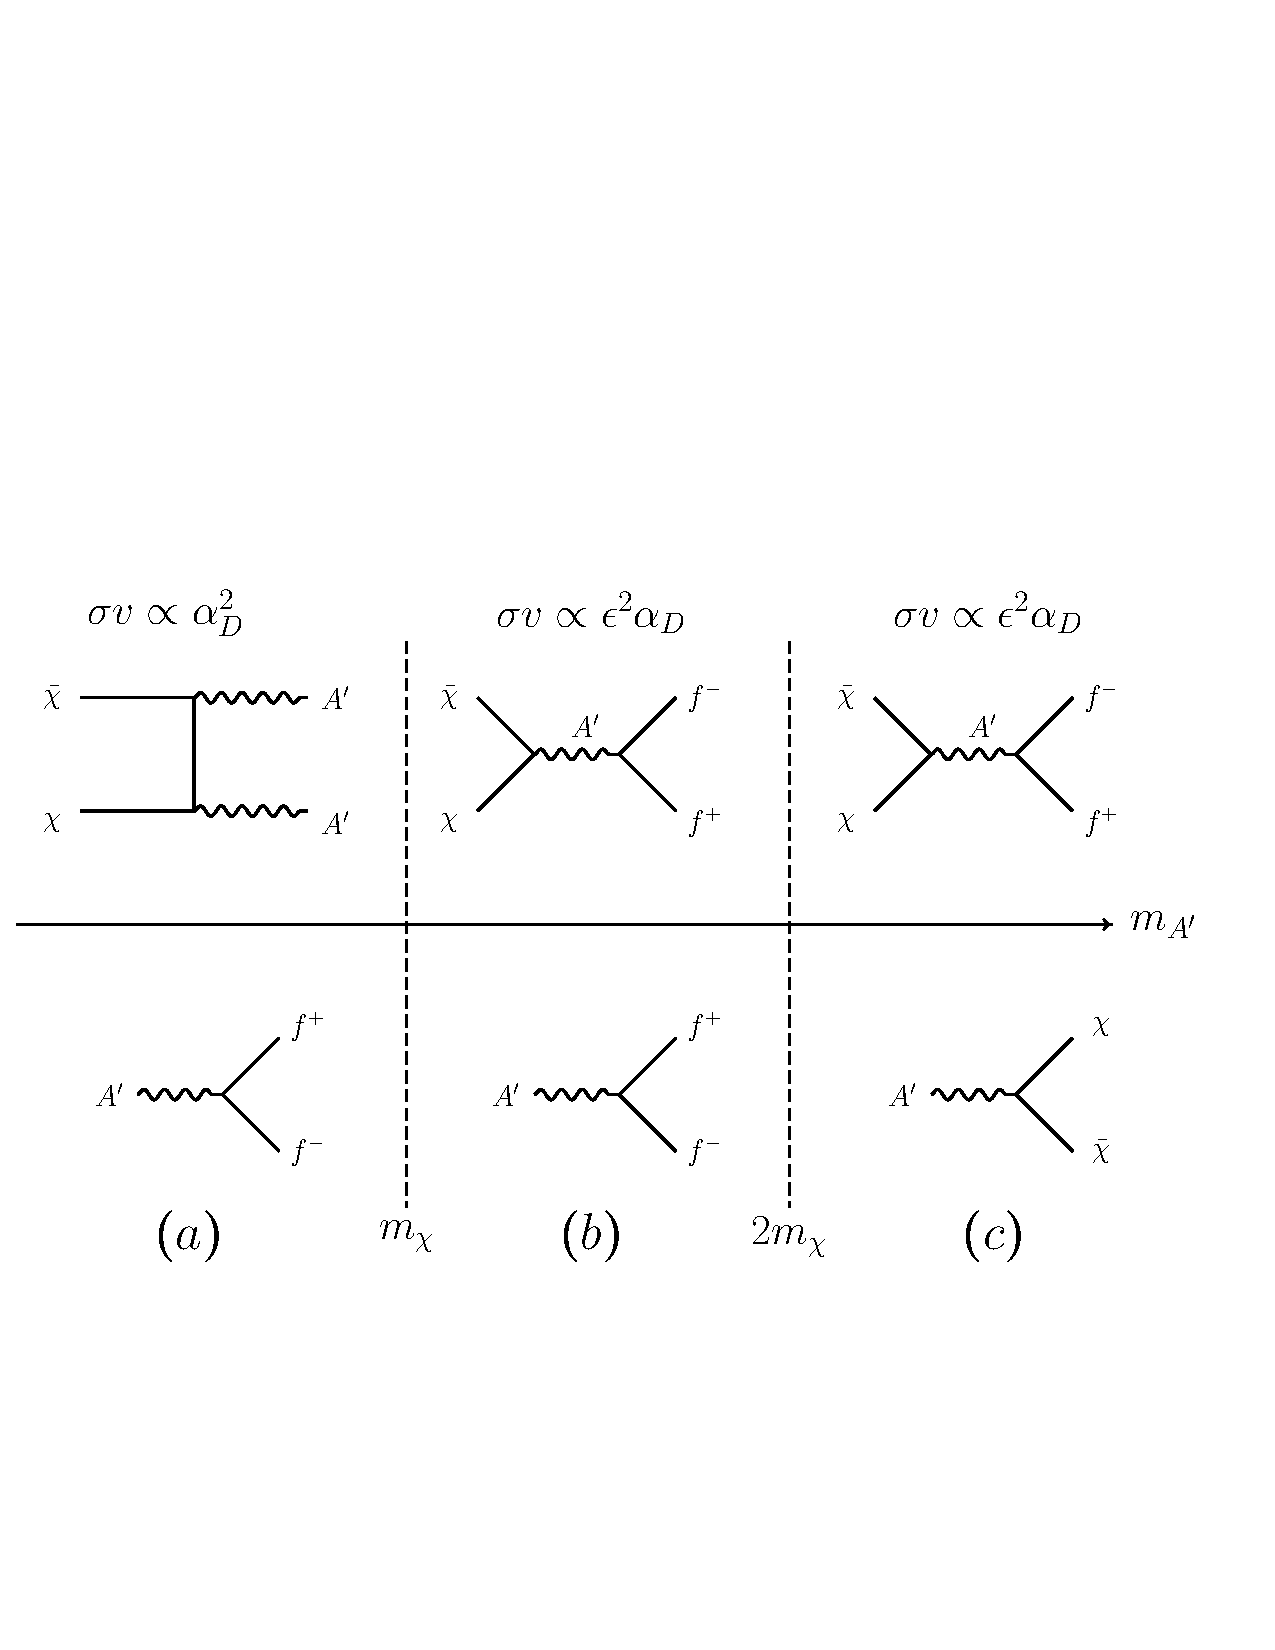
\includegraphics[width=15cm]{breakdown.pdf}
\caption{ Schematic representation of the different DM annihilation modes (top row) and $A'$ decay modes for $m_\chi/m_{A^\prime}$ ratios. 
a) Secluded annihilation scenario with  a visibly decaying mediator. This scenario has no thermal target and cannot be presented on
the $y$ vs. $m_\chi$ plane. b) Compressed region with direct annihilation, but a visibly decaying mediator (not considered in this discussion). c) 
Direct annihilation and invisibly decaying mediator particle.    }
\label{fig:phases}
\end{figure}


\subsection{Predictive LDM Targets}
We define the LDM particle to be $\chi$ and the mediator to be  a ``dark photon" $A^\prime$ with lagrangian 
\be
{\cal L} = i \bar \chi \displaystyle{\not}{\,\partial} \chi + m_\chi \bar \chi \chi + g_D A^{\prime}_\mu \bar \chi \gamma^\mu \chi -\frac{1}{4} F^\prime_{\mu \nu}{F^\prime}^{\mu \nu}     + \frac{\epsilon}{2} F^\prime_{\mu \nu}F^{\mu \nu}  
 + \frac{m_{A^\prime}^2}{2}  A^\prime_\mu  {A^\prime}^\mu ~,~
\ee
where $F^\prime_{\mu\nu} = \partial_\mu A^\prime_\nu - \partial_\nu A^\prime_\mu$,  $\epsilon \ll$ is the kinetic mixing parameter, which controls $A^\prime$ mixing with the SM photon, and $g_D \equiv \sqrt{4\pi \alpha_D}$ is the  $A^\prime$ coupling to the DM. Although we've assumed the DM is a fermion, the qualitative features
of this discussion are insensitive to its spin and compatible with scalar candidates as well.  

After diagonalizing the kinetic mixing interaction, the dark photon $A^\prime$  acquires a coupling to the SM electromagnetic current 
\be
{\cal L} \to  i \bar \chi \displaystyle{\not}{\,\partial} \chi + m_\chi \bar \chi \chi +A^{\prime}_\mu \biggl( g_D  \bar \chi \gamma^\mu \chi  + \epsilon e \sum_f Q_f \bar f \gamma^\mu f \biggr)  -\frac{1}{4} F^\prime_{\mu \nu}{F^\prime}^{\mu \nu}  
 + \frac{m_{A^\prime}^2}{2}  A^\prime_\mu  {A^\prime}^\mu ~,~
\ee
where $f$ is a SM fermion and $Q_f$ is its electromagnetic charge.

We distinguish between two distinct annihilation regimes depicted schematically in Fig. \ref{fig:phases}
 \begin{itemize}
  \item {\bf Secluded Annihilation:} For $m_{A^\prime}  < m_{\chi}$, DM annihilation will predominantly proceed through $\chi \chi \to A^\prime A^\prime$, followed
   by $A^\prime \to ff$ decays to SM fermions. However, the annihilation rate in this regime is independent of the SM-$A^\prime$ coupling $\epsilon$ and therefore difficult to test since thermal freeze out can proceed even for
  tiny values of $\epsilon$. This regime is depicted on the leftmost column of Fig. \ref{fig:phases}
 
 \item  {\bf Direct Annihilation:} For $m_{A^\prime} >  m_{\chi}$, the mediator decays predominantly to DM and annihilation 
 proceeds via  $\chi \chi \to {A^\prime}^* \to ff$ to SM fermions $f$ through a virtual mediator. This regime is depicted in the middle and rightmost column of Fig. \ref{fig:phases};
 ; note the compressed region in the middle column for which $m_\chi < m_{A^\prime} < 2 m_\chi$ for which
   the annihilation rate depends on $\epsilon$ but the mediator decay to DM is kinematically forbidden.
\end{itemize}

Since the cross section for direct annihilation is proportional to all the parameters in the DM lagrangian, it is convenient
to define the dimensionless interaction strength $y$ as
\be
\sigma v (\chi \chi \to {A^\prime}^*  \to f f) \propto  \epsilon^2 \alpha_D \frac{m_\chi^2}{m_{A^\prime}^4} =  \frac{y}{m_\chi^2}~~~~,~~~~ y \equiv 
\epsilon^2 \alpha_D  \left(     \frac{m_\chi}{m_{A^\prime}  }    \right)^4
\ee
thus, for each choice of $m_\chi$ there is a unique value of $y$ compatible with thermal freeze out independently of the individual
values of $\alpha_D, \epsilon$ and $m_\chi/m_{A^\prime}$. Reaching experimental 
sensitivity to this benchmark for masses between 10 keV -- GeV suffices for decisive coverage of these scenarios.

\subsection{Current Bounds on LDM}


\begin{figure}[t!]
\center
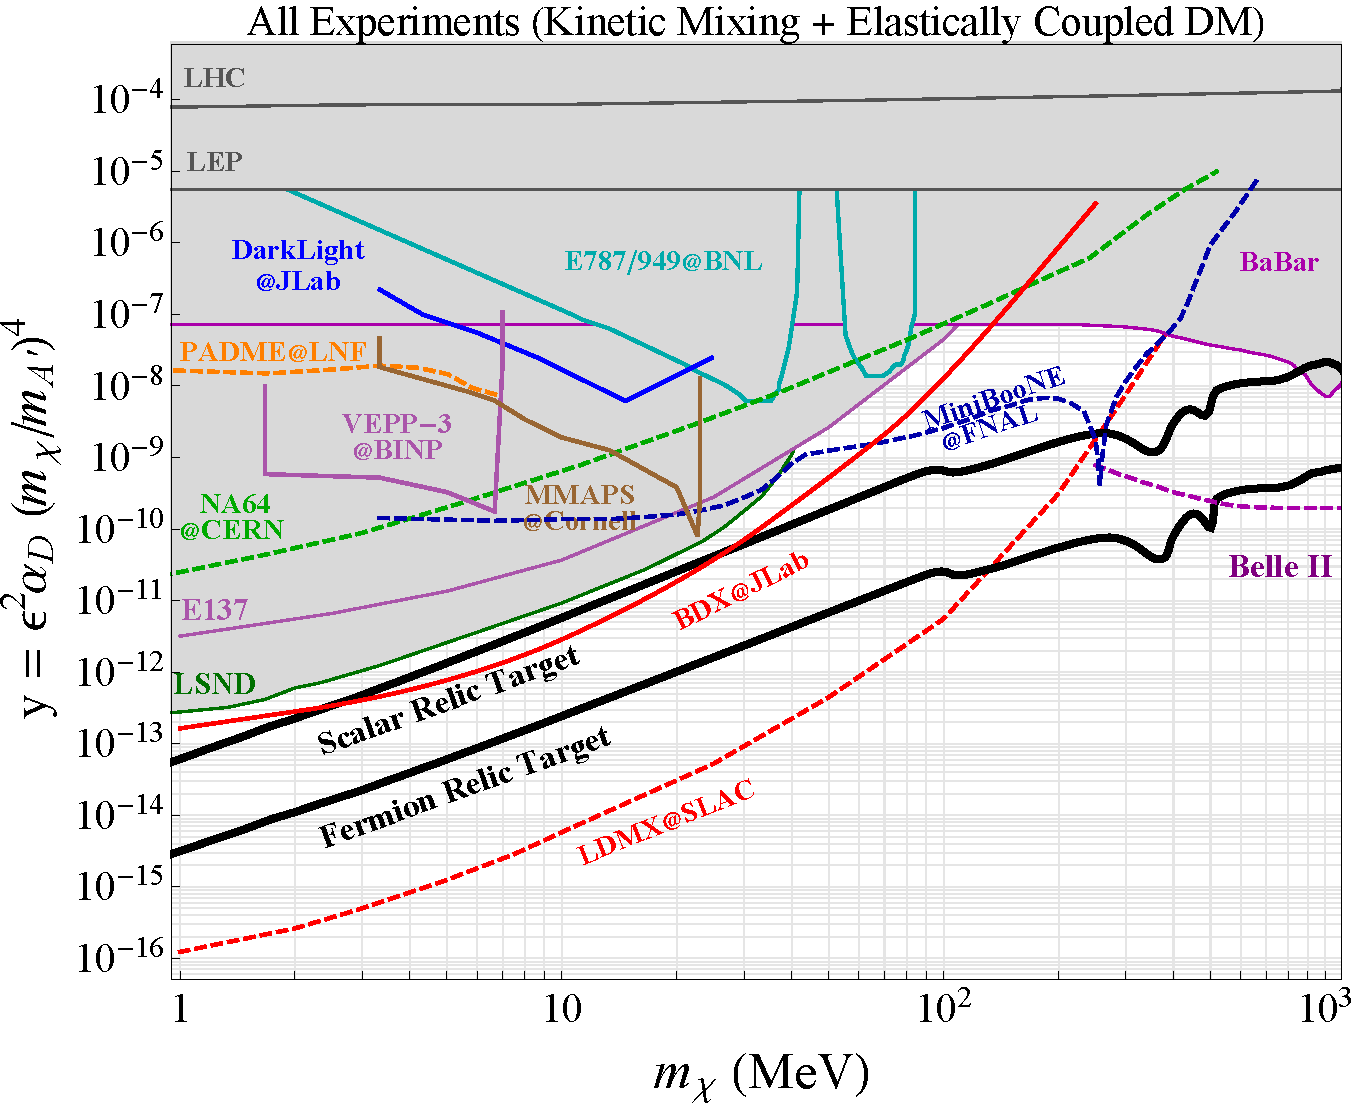
\includegraphics[width=11cm]{everything.pdf}
\caption{ The parameter space for LDM and future experimental projections in the $y$ vs. $m_\chi$ plane plotted against
 the thermal relic targets for scalar and fermion DM -- see text for a discussion. }
\label{fig:mainplot}
\end{figure}

2
Although LDM represent fully half of the viable thermal DM mass range, there has never been a dedicated search
for this class of models. Most constraints that apply to the scenarios considered here are reinterpretations (by theorists)
of experimental results collected for other purposes and fall into the following categories:

\begin{itemize}

\item {\bf CMB Power Spectrum:} LDM can annihilate to SM particles during the time of recombination and ionize the newly 
formed hydrogen, thereby modifying the CMB power spectrum in conflict with observations from PLANCK \cite{dodge}. 
If this annihilation is $s$-wave and the DM is particle symmetric, the CMB rules out  LDM below $\sim $10 GeV. However
if the annihilation is $p$-wave (easily achieved for a scalar DM candidate coupled to a dark photon mediator) or 
if the DM population is different at the time of CMB (e.g. asymmetric or Majorana inelastic, see \cite{Izaguirre:2015yja} for a discussion)  
 
\item {\bf Colliders:} Although high energy colliders (LHC, Tevatron, LEP) generally have poor sensitivity to LDM, high intensity B-factories 
can perform analogous searches for $e^+e^- \to \gamma A^\prime$ production and set impressive constraints in the 100 MeV - few GeV 
mass range. 

\item {\bf Beam Dumps: } The LSND proton beam dump experiment  \cite{deNiverville:2011it} is sensitive to LDM production and scattering
in their measurement of the electron-neutrino neutral current cross section. At LSND, DM can be produced in pion decays $\pi^0 \to \gamma A^\prime \to \gamma \chi \chi$
and subsequently scatter in a downstream detector.  The E137 electron beam dump experiment  to search for axion like particles is also sensitive to 
similar processes in which DM is relativistically  produced through the kinetic mixing interaction in the beam dump, passes through a downstream 
 detector and deposits electromagnetic energy by scattering off detector targets  \cite{Batell:2014mga}. 

\item{\bf Rare Kaon Decays}: LDM can also be produced in rare Kaon decays $K^+ \to \pi^+ A^\prime \to \pi^+ \chi \chi$ which 
can contribute to the signal region of E787/E949  \cite{Adler:1997am,Artamonov:2008qb} which measured the $K^+ \to \pi^+ \bar \nu \nu$ branching ratio. 

\item{\bf Electron Direct Detection}: The results of XENON10 S2-only study of electron recoil signals can be used to 
constrain LDM that scatters elastically off detector electrons \cite{Essig:2012yx}. Although the backgrounds for this sample are not well understood,
a conservative extraction of the DM scattering limit can be used to constrain this parameter space. This bound is competitive with 
E137 and E787/E949 in Fig. \ref{fig:main plot}, but is slightly covered by those constraints for the benchmarks presented, so it is not shown.

\end{itemize}

These constraints are collected in on the $y$ vs $m_\chi$ parameter space depicted in Fig. \ref{fig:mainplot}  alongside projections
for Belle II \cite{Essig:2013vha}, BDX \cite{Izaguirre:2013uxa,Battaglieri:2016ggd}, MiniBooNE \cite{Dharmapalan:2012xp}, NA64 \cite{Gninenko:2016kpg}, VEPP-3 \cite{Wojtsekhowski:2012zq}, and MMAPS \cite{cornell}.
Also shown are the thermal targets for fermion and scalar LDM candidates, which are invariant in this parameter space regardless
of what assumptions about $\epsilon, \alpha_D$, and $m_\chi/m_{A^\prime}$ we choose. However, the other constraints on this 
parameter space are not necessarily invariant in this way (e.g. collider production only depends on $\epsilon$), so the 
shaded regions in Fig. \ref{fig:mainplot} represent the most conservative versions of these constraints for which
 these parameters are chosen to reveal all the remaining gaps in the parameter space consistent with the assumption of 
 direct annihilation. 
 
 This plot illustrates the large, orders of magnitude gaps in coverage between existing (and projected) constraints
 and the thermal relic contours for LDM. In order to decisively cover thermal LDM in the direct annihilation regime, a dedicated effort will
 be required. To this end, we also show the projections for LDMX@SLAC, which is the only proposed effort to probe the thermal
 target for both scalars and fermions down to the MeV range. 

\bibliography{MotivationBib}

\end{document}
